\section{Les pages Web}
biblio
https://www.w3.org/TR/html5/ \\
https://fr.wikipedia.org/wiki/HTML5 \\
https://fr.wikipedia.org/wiki/Hypertext\_Markup\_Language

http://adiguba.developpez.com/tutoriels/j2ee/jsp/jstl/\#L1.1
http://www.objis.com/formation-java/tutoriel-jstl-installation-jakarta-taglib.html

%%%%%%%%%%%%%%%%%%%%%%%%%%%%%%%%%%%%%%%%%%%%%%%%%%%%%%%%%%
%----------------------HTML/CSS--------------------------%
%%%%%%%%%%%%%%%%%%%%%%%%%%%%%%%%%%%%%%%%%%%%%%%%%%%%%%%%%%
\subsection{HTML, CSS et JavaScript}
Pour créer nos pages web nous allons utiliser le langage HTML5. Généralement, lorsque l'on parle d'HTML5 cela comprend également le CSS3 et le JavaScript, qui forment à eux trois des technologies Web permettant de développer des applications.
\begin{figure}[H]
  \center
  
\includegraphics[scale=0.6]{../graph/html5.png} \\
  \caption{ \url{https://fr.wikipedia.org/wiki/HTML5}}
\end{figure}

Le HTML est un langage de balisage qui permet d'écrire de l'hypertexte, ces balises permettent de structurer les pages Web et on peut également y inclure du contenu multimédia (images notamment). On utilise en parallèle le CSS afin de faire un format uniforme qui est fonction le plus souvent des balises. Ainsi, la feuille de style (.css) qui est créée peut être appliquée à toutes les pages Web et on obtient alors un site avec un format homogène et ce en ayant un code léger puisqu'on n'a pas besoin de s'occuper du format au sein de chaque page mais seulement de faire attention aux balises utilisées.\\

Par ailleurs, on a dit que l'on pouvait intégrer du code écrit en JavaScript dans les pages HTML. Cela peut permette notamment de personnaliser la page et de réagir à certaines actions de l'utilisateur. Par exemple, il existe un évènement 'OnMouseOver' qui se déclanche lorsque l'on passe la souris sur un élément de la page, on peut alors choisir la réaction que va avoir la page Web. Un exemple simple est lorsque l'on passe sur une image, elle grossit. \\

JavaScript permet également de faire des choses comme le calendrier que nous allons utiliser dans notre application. En effet, nous avons besoin de faire choisir à l'utilisateur des dates, pour qu'il saisisse une date valide directement, nous avons préféré lui proposer un calendrier. Pour cela, Javascript est un bon outil. Dans l'exemple qui suit, l'utilisateur cliquera dans la case blanche réservée à la saisie d'une date et verra s'afficher le calendrier en-dessous. On peut remarquer par ailleurs que le calendrier est personnalisé : nous avons utilisé le langage CSS afin d'utiliser le même format pour le calendrier que pour les pages.
\begin{figure}[H]
  \center
  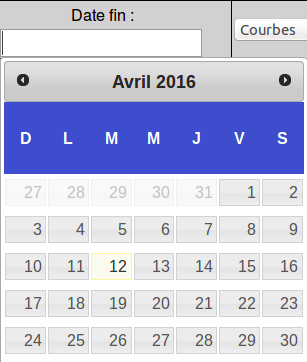
\includegraphics[scale=0.5]{../graph/JavaScriptCalendrier.png} \\
  \caption{Exemple d'utilisation de JavaScript pour afficher des éléments intéractifs dans la page Web.}
\end{figure}

JavaScript nous servira également lorsque nous voudrons ajouter des graphiques à nos pages Webs et cela en utilisant un API Google Chart qui sera intégrée à l'application via le langage JavaScript.

%%%%%%%%%%%%%%%%%%%%%%%%%%%%%%%%%%%%%%%%%%%%%%%%%%%%%%%%%%
%----------------------JSTL------------------------------%
%%%%%%%%%%%%%%%%%%%%%%%%%%%%%%%%%%%%%%%%%%%%%%%%%%%%%%%%%%
\subsection{La libraire JSTL}
Comme nous l'avons vu précédemment, nous utilisons des pages JSP qui permettent de créer des pages Web dynamiques et ce notamment en y incorporant du code Java. Afin de faciliter l'écriture des JSP et aussi de les rendre plus 'propres', on peut utiliser des \textbf{tags}. La librairie JSTL (Java Standard Tags Librairy) procure un certain nombre de tags prédéfinis.\\

On intègre à nos JSP cette librairie avec la ligne suivante en tout début de page (avant les balises <HTML>). Cela permet alors d'utiliser les tags (simples) de la librairie. Si on veut utiliser d'autres tags de format ou fonctions, il faut intégrer les deux lignes suivantes.
\begin{lstlisting}[language=XML]
<%@ taglib uri="http://java.sun.com/jsp/jstl/core" prefix="c" %>
<%@ taglib uri="http://java.sun.com/jsp/jstl/functions" prefix="fn" %>
<%@ taglib uri="http://java.sun.com/jsp/jstl/fmt" prefix="fmt" %>
\end{lstlisting}  

Il existe tout un ensemble de balises, si l'on cite les plus importantes, on aura :\\

\noindent
\begin{tabular}{|l|l|}
  \hline
      <c:\textbf{set} var="un" value="1"/> 		& Déclarer des variables. \\ 
  \hline 
      <c:\textbf{import} url="/inc/menu.jsp" /> 	& Importer une autre page JSP. \\
  \hline 
      <c:\textbf{if} test="boolean"></c:\textbf{if}> 	& Exécuter un test. \\
  \hline        					    
      <c:\textbf{forEach} var="var" items="tableau" >> 	& Exécuter une boucle sur un tableau ou une autre structure, \\
      </c:\textbf{forEach}				& la variable var est une sorte d'itérateurs sur la structure. \\
  \hline        					    
\end{tabular}
